%% ============================================================
%% Rozdział 3 — Wyniki
%% ============================================================
\chapter{Wyniki}\label{chapter:3_Results}
W niniejszym rozdziale należy przedstawić wyniki uzyskane w trakcie realizacji pracy dyplomowej. Powinny one stanowić logiczne rozwinięcie części teoretycznej oraz metodyki projektowej. Opis powinien zawierać przedstawienie uzyskanych rezultatów. Należy także wyjaśnić, co one oznaczają, czyli przedstawić ich interpretację. W opisie trzeba ocenić uzyskane wyniki, wskazując ich znaczenie i wiarygodność. Dobrze jest również porównać je z innymi rozwiązaniami, danymi teoretycznymi lub z oczekiwanymi rezultatami. W zależności od charakteru pracy, w tym rozdziale można również zamieścić szczegółowy wykaz zastosowanych metod, narzędzi lub technologii, a także przykłady ich wykorzystania w praktyce.

\section{Elementy ilustracyjne  i analiza wyników}
\noindent Ten podrozdział przedstawia przykładowe sposoby prezentacji wyników, obejmujące:
\begin{itemize}
  \item wzory matematyczne (z numeracją po prawej stronie kolumny),
  \item rysunki (z podpisem pod ilustracją, numeracją ciągłą),
  \item tabele (z tytułem nad tabelą i jednostkami w osobnej kolumnie),
  \item a także zasady odwoływania się do tych elementów w tekście.
\end{itemize}

\noindent Poprzez polecenie \verb|\noindent|, możliwe jest kontynuowanie akapitu (bez wcięcia).

%% ------------------------ Wzory ------------------------------
\subsection{Edycja wzorów}
Wzory matematyczne należy wstawiać przy użyciu środowiska  \verb|equation|, które automatycznie nadaje numerację, np.:
\begin{equation}
\label{eq:linear_equation}
\mathbf{A}x=b,
\end{equation}
\noindent gdzie:

\vspace*{0.5em}
\begin{tabular}{@{}lll}
$\mathbf{A} \in \mathbb{R}^{n\times n}$ &- &macierz współczynników,\\
$x \in \mathbb{R}^{n}$         &-&wektor niewiadomych,\\
$b \in \mathbb{R}^{n}$         &-&wektor wyrazów wolnych.
\end{tabular}
\vspace*{0.5em}

\noindent Do każdego wzoru należy odwoływać się w tekście za pomocą polecenia \verb|\eqref{}|, jak pokazano w równaniu \eqref{eq:linear_equation}. Wszystkie symbole użyte we wzorze powinny być jednoznacznie wyjaśnione bezpośrednio pod nim. Zmienne i wielkości fizyczne należy zapisywać kursywą, np. $x$, natomiast macierze i wektory – pogrubionym fontem matematycznym, np. $\mathbf{A}$. Należy również pamiętać o zasadach zapisu wartości liczbowych (bez odstępu przed znakiem minus), np. $-$20 oraz o oddzielaniu jednostek spacją, np. 5 V lub poleceniem \verb|\:| wewnątrz operatora matematycznego np. 10$\: \frac{\mathrm{m}}{\mathrm{s^2}}$. Jeśli jest to możliwe, należy unikać wstawiania równań bezpośrednio w tekście akapitu. W przypadku potrzeby przedstawienia układu równań, można użyć środowiska \verb|cases|:
\begin{equation}
\begin{cases}
x + y = 5,\\
2x - y = 1.
\end{cases}
\label{eq:uklad}
\end{equation}
\enlargethispage{\baselineskip}

%% ------------------- Wykresy i grafika ----------------------
\subsection{Wykresy i grafika}
Każdy wykres lub rysunek powinien mieć numer oraz podpis umieszczony pod ilustracją. Należy zwrócić uwagę, aby zachować odpowiednią wielkość czcionki (Arial 9 pt), proporcje osi i ogólną estetykę wykresu. Zaleca się stosowanie formatów wektorowych (np. .eps, .pdf, .svg), ponieważ umożliwiają one zachowanie pełnej jakości podczas skalowania. Należy unikać grafik rastrowych (np. .png, .jpg) pochodzących ze zrzutów ekranu o niskiej rozdzielczości. Rysunek należy wstawić, wykorzystując środowisko \verb|figure| z opcją \verb|[!htbp]|, aby utrzymać jego pozycję w danym miejscu tekstu, np.:

\begin{figure}[!htbp]
  \centering
  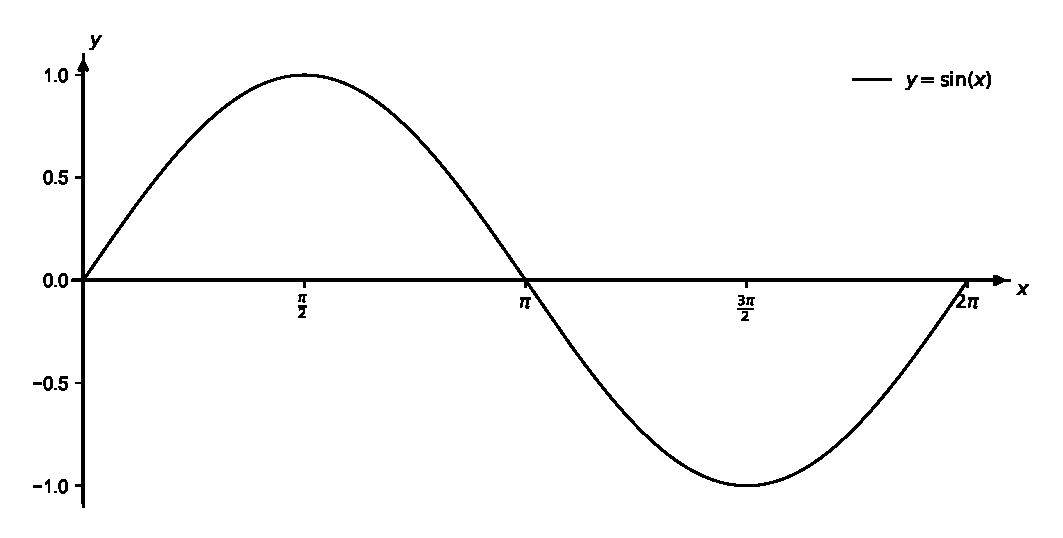
\includegraphics[width=1\linewidth]{img/sin.eps}
  \caption{Wykres funkcji sinus. Kod programu w Pythonie wykres znajduje się w Dodatku \ref{page:A_appendix}.}
  \label{fig:sin}
\end{figure}

\noindent LaTeX automatycznie generuje spis rysunków po użyciu polecenia \verb|\listoffigures|. W przypadku użycia materiałów zewnętrznych (np. zdjęć, wykresów, schematów) należy wskazać źródło oraz upewnić się, że nie narusza to praw autorskich.

%% ------------------------- Tabele ---------------------------
\subsection{Tabele}

W pracy inżynierskiej warto stosować tabele (umieszczane w środowisku \verb|table|) przedstawiające zestawienia parametrów technicznych, wyniki pomiarów, konfiguracje systemów lub porównania wydajności. Tytuł umieszczony jest nad tabelą (polecenie \verb|label|). Jeśli tabela jest bardzo szeroka, można zastosować polecenie: \verb|\resizebox{\textwidth}{!}{...}| lub pakiet \verb|longtable| dla tabel na kilka stron. Należy pamiętać o odwołaniu się do tabeli w tekście poprzez polecenie \verb|\ref{}|.

\begin{table}[!htbp]
\centering
\caption{Zestawienie podstawowych parametrów systemu testowego}
\label{tab:test_params}
%% @{} -> usuwa wewnętrzny odstęp przy lewej/prawej krawędzi tabeli
%% \raggeright wyrównuje do lewej
%% p{.28\linewidth} -> kolumna o stałej szerokości 28% szerokości tabeli
%% X wypełnia pozostałą szerokość; łamie wiersze jak p{...}
%% >{\centering\arraybackslash}p{.13\linewidth} -> kolumna o stałej szerokości 13% szerokości tabeli wyśrodkowana;
%% \arraybackslash przywraca ustawienia domyślne na końcu komórki
\begin{tabularx}{\linewidth}{@{}>{\raggedright}p{.28\linewidth}>{\raggedright\arraybackslash} X
                              >{\centering\arraybackslash}p{.13\linewidth}
                              >{\centering\arraybackslash}p{.13\linewidth}@{}}
\textbf{Parametr} & \textbf{Opis} & \textbf{Wartość} & \textbf{Jednostka} \\ \hline
Częstotliwość taktowania & Główna częstotliwość zegara mikrokontrolera & 80 & MHz \\
Napięcie zasilania & Wartość napięcia wejściowego & 5,0 & V \\
Pobór prądu & Średni pobór prądu podczas pracy & 120 & mA \\
Temperatura pracy & Zakres bezpiecznej pracy urządzenia & $-$10 – 60 & °C \\
Czas próbkowania & Interwał pomiarowy w pętli głównej & 50 & ms \\
Liczba kanałów wejściowych & Liczba obsługiwanych czujników analogowych & 8 & – \\
Typ transmisji danych & Protokół komunikacyjny używany do transmisji & UART & –
\end{tabularx}
\end{table}
\FloatBarrier

%% ----------------- Zakończenie rozdziału --------------------
\section{Podsumowanie rozdziału}
Rozdział z wynikami powinien kończyć się krótkim podsumowaniem najważniejszych obserwacji i wniosków płynących z analizy. Warto również wskazać potencjalne ograniczenia badań lub obszary wymagające dalszych testów i porównań.
